\chapter{Connect Hydro Project}
\markright{Connect Hydro Project}
\label{ChapterThree}
In this chapter, We will discuss what are hydro power plants, how they work and their different sizes, their electricity generating menthods(types) along their advantages and disadvantages. Also, We will discuss the control strategies that can be used for hydro power plants. Finally the Connect Hydro Porject will be discussed in terms of its aspects and proposed concept. And finally give  we will give an overview of the proposed implementation for the Connect Hydro Project.
\section{Small Hydro Power Plants}
\label{SmallHydroPowerPlants}
Hydro power plants make use of the the power of moving water to produce electricity or mechanical energy. There exists two key factors for effective hydro power generation, they are “head” and “flow.” “Head” refers to the height over which the water falls, while “flow” refers to the volume of water per unit time.\cite{SmallScale} To maximise energy production, both head and flow should be high. In other words, the larger volume of water flowing over a steep gradient the greater amount of energy is generated. In small hydro power stations, it is important that a proper height of water fall is obtained naturally without building elaborate and expensive facilities.\cite{SmallScale,HydroPower} A well designed small hydropower system can blend with its surroundings and have minimal negative environmental impacts.\cite{SmallScale,HydroPower}\\

\textbf{Hydroelectricity} is a term that refers to electricity generated by hydro power plants. The electricity produced may be used directly, stored in batteries, or inverted to produce utility-quality electricity. Hydropower plants generate Hydroelectricity by directing water through a turbine, which in turn drives an electric generator. It is the most widely used form of renewable energy, accounting for 16 percent of global electricity generation – 3,427 terawatt-hours of electricity production.\cite{HydroPower}

Hydro Power technology is extremely robust (systems can last for 50 years or more with little maintenance) and is also one of the most environmentally benign energy technologies available.\cite{paish2002small} Figure 3.2 shows an example of a small hydro power plant. In the following sections we will discuss the different types of hydro power stations and how they generate electricity as well as the advantages and disadvantages of small hydro power plants.
\begin{figure}[H]
\centering
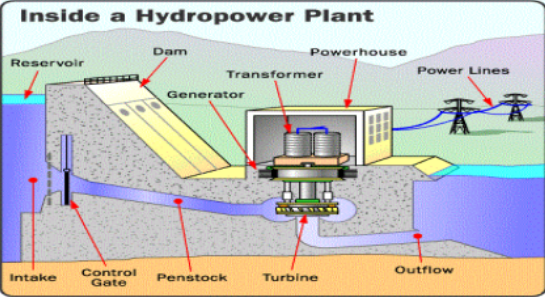
\includegraphics[scale=0.7]{Images/GeneralPowerPlant.png}
\caption[General Power Plant Structure]{General Power Plant Structure \cite{HydroPP}}
\end{figure}
The classification of Hydro power plants is acheived according to their average energy output, expressed in megawatts.\cite{HydroPP} As shown in Figure 3.1, large scale hydro power plants produce more than 100 MW, Medium Scale hydro power plants produce energy between 10-100 MW, small hydro power plants produce less than 10 MW.\cite{HydroPP,SEIT2017} Based on energy production capacity, small-scale hydropower production is broken into four size categories of pico- (<5 kilowatts), micro- (5-100 kW), mini- 100 kW-1 MW), and small (1-10 MW).\cite{HydroPP}

There doesn't exists a common consensus among countries about the classifications of hydro power plants. For instance, some European Union countries like Portugal, Spain, Ireland, Greece and Belgium accept 10 MW as the upper limit for small-scale hydropower installed capacity, while others place the maximum capacity from 3 to 1.5 MW. Outside the EU, this limit can be much higher, as in the USA (30 MW) and India (25 MW).\cite{HydroPP}
\begin{figure}[H]
\centering
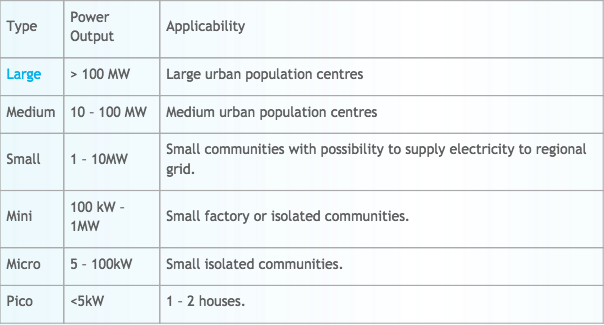
\includegraphics[scale=0.7]{Images/PP_Classification.png}
\caption[Power Plant Size Classification]{Power Plant Size Classification \cite{HydroPower}}
\end{figure} 
\subsection{Advantages of Small Hydro Power Plants}
Hydro electric energy is a renewable electrical energy source. Hydro Power Plants don't produce any heat or toxic gases and therefore considered non-polluting. They have a low operating, maintenance cost as well as no fuel cost which makes it inflation proof. They offer reliable and flexible operation with a long life. Many existing stations have been in operation for more than half a century and are still operating efficiently. Hydro power station produce energy with an efficiency of over 90\%, it the most efficient of energy conversion technologies. Finally, Hydro power offers a quick means of responding to changes in load demand or due to certain events.\cite{SmallScale}
\subsection{Disadvantages of Small Hydro Power Plants}
One of the drawbacks of small hydro power stations are their limitations in regards of their placement. They need to be in a location that is near the electrical power grid so that the electricity generated can be used and taken advantage of. Small power plants are limited by the river/stream water flow, they have a maximum capacity which cannot be exceeded even with high water flow. The energy supply is also disturbed by changing seasons; Yearly planning must be done to ensure constant power generation as they must be shutdown in the case of low water level.\cite{HydroPP,SEIT2017} They are also sussepctable to have problems with suspended loads (foilage, branches, waste) which requires flushing; the process of removing foilage from water by the trash racks before entering the turbine.\cite{SEIT2017}
\subsection{Small Hydro Power Plants Types}
\begin{itemize}
\item \textbf{Conventional (dams):} Hydro electric power comes from the potential energy of water saved before a dam which is then used by the water turbine and generator to generate electricity. The electricity output relies on the volume and the difference in height between the dam and the water's outflow also known as the "Head". The higher the head, the higher the amount of potential energy in the water, they are proportional. A large pipe (the "penstock") delivers water to the turbine.\cite{HydroPP} 
\item \textbf{Pumped-storage:} This method produces electricity by moving water between reservoirs at different levels. At times of low energy demand, excess energy is used to pump water back into higher reservoirs. Whereas at times of higher demand, water is moved back into the lower reservoir through a turbine.\cite{HydroPP} Pumped-storage are the most commercially implemented means of large-scale grid energy storage and improve the daily capacity factor of the generation system.\cite{HydroPP}
\item \textbf{Run-of-the-river:} In run-of-river systems, river water is diverted by a weir through an opening in the river side (the ‘intake’) into a channel.\cite{HydroPower} A sandtrap is built in the channel to remove sand and leaves from the water. Water in directed through the into a small reservoir/tank known as the ‘forebay’ from where it is directed on to the turbines through a closed pipe known as the ‘penstock’.\cite{HydroPower} The penstock's main functionality is to direct the water in a constant stream to the turbine at a lower level. Power generated by the turning shaft of the turbine can be used to rotate a mechanical device (such as a grinding mill, oil expeller, or wood lathe), or to operate an electricity generator.\cite{HydroPower} When electricity is generated, the ‘power house’ where the generator is located, transfers the electricity to a step-up ‘transformer’ which is then transmitted to the electricity grid. Water is returned back to the river after the electricity is produced by the turbine.\cite{HydroPower} Figure 3.3 shows a diagram of how a run-of-the-river powerplant is built.

Most small hydro power plants are “run-of-the-river” types. The turbines are turned on to generate electricity only when the water level at the river/stream is high enough.
\begin{figure}[H]
\centering
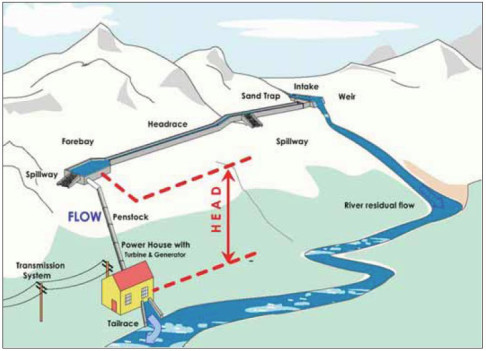
\includegraphics[scale=0.7]{Images/RunOfRiver.jpg}
\caption[Run of the River Example]{Run of the River Example \cite{HydroPower}}
\end{figure}
\item \textbf{Tidal:} A tidal power plant exploits the fact that there is a daily rise and fall of ocean water due to tides; which are highly predictable. In some sitiuations, construction of reservoirs is permitted and can be used to generate power during high demand periods even if the tides are not high. Tidal power can only be exploited in a relatively small number of locations around the world.\cite{HydroPP}
\item \textbf{Underground:} An underground power station can only be constructed in a place where there exists a large natural height difference between two waterways, such as a waterfall or a mountain lake. Water is taken from the high reservoir to the generator room that is uaually built in an underground cavern near the lowest point of the water tunnel through nn underground tunnel. Water is then released back to the lower outlet waterway.\cite{HydroPP}
\end{itemize}
\section{Control Strategies}
One of the problems facing small hydro power plants  located along the same river is lack of communication between the owners. This lack of communication results in less efficiency in energy production. The main problem emerges when one owner does a certain action that affects the successor powerplants but fails to communicate it.\cite{SEIT2017} Most research articles propose concepts and cooperation techniques to increase energy production and communication between large power plants.\cite{SEIT2017}. Jäger et al.\cite{SEIT2017} discussed different control strategies that are relevant to small hydro power plants. These control strategies will be discussed in this section.

 In this section, we will work under the assumption that a series of small hydro power plants operating on one river can be viewed as a linear system with a defined neighborhood.\cite{farina2012distributed} The neighborhood of one subsystem can be specified as a set of directly affecting subsystems of the whole linear system.\cite{farina2012distributed} A control strategy can be defined as the essential characteristics of how the distributed subsystems (the plants) in such a linear system are controlled. A classification of distributed Model Predictive Control (MPC) proposed by Farina \cite{farina2012distributed} based on:\\
\indent • the information exchange protocol, i.e., non-iterative or iterative,\\
\indent • the type of the cost function to be optimized, i.e., cooperative or non-cooperative, and\\
\indent • the topology of the transmission network, i.e., fully connected or partially connected.

There can exists two implementations of such distributed MPCs, a third centralized approach is introduced by Jäger et al.\cite{SEIT2017} They are \cite{SEIT2017}:
\begin{itemize}
	\item The Local Control Strategy (LCS): A strategy based on a non-iterative and non-cooperative approach, which allows for only a partially connected topology.
	\item The Collaborative Control Strategy (CCS): As strategy that uses a cooperative approach, which relies on a fully connected topology of the transmission network.
	\item The Centralized Control Strategy (CCS): A strategy that uses information from all partners in the overall system and supplies them with the control details. A centralized service is created where every partner has to connect to this service. The service in turn coordinates all partners with respect to defined individual and the overall goals.
\end{itemize}
\subsection{Local Control Strategy}
The concept that the local control strategy is based on, is that the control of the individual subsystem depends on data from other subsystems. All subsystems are data consumers and data providers\cite{SEIT2017}. No coperation between the subsystems is considered, each subsystem is controlled locally. 

Farina et al.\cite{farina2012distributed} proposed their distributed predictive control schema for linear discrete-time systems, which focuses on non-iterative, non-cooperative, partially connected, to solve this kind of a distributed MPC problem. The approach relies on neighbours sending or receiving information at each sampling time about their future reference trajectories, and guarantee that the actual ones lie within a certain range of the reference ones.\cite{SEIT2017} Following that, each subsystem solves its own optimization problems. A two-phase approach was proposed by Matz et al. 9 to optimize the control of a single plant. The first phase involved optimizing the plant control ”off-line”, i.e., all predictions and decisions are based on historical data only.\cite{SEIT2017} The second phase also includes the prediction based on current, if possible real-time data and/or predictions. With this approach, additional data from the neighbors can be integrated into the individual control. This strategy utilizes the neighbor-to-neighbor communication and provides some profit to selected partners via decentralized optimization within the linear system even if not all partners in the line are contributing their information.\cite{SEIT2017} 
\subsection{Cooperative Control Strategy}
Unlike the local control strategy, in the cooperative control strategy, all subsystems are required to consider the effects of local control actions on them. Each subsystem is required to optimize for an objective defined for the overall system. Stewart et al.\cite{stewart2010cooperative} propose the use of state and output feedback to improve the overall performance. The cooperative control strategy is frequently used within one plant, integrating the different systems, to achieve an optimal overall objective.\cite{SEIT2017,stewart2010cooperative}
\subsection{Centralized Control Strategy}
In the centralized control strategy, a centralized service is created that controls all subsystems, optimizing towards a centralized controller objective\cite{SEIT2017}. Control information is sent and recieved by all systems from the service. A powerful centralized server with strong optimization software are the main advantages of this apprach. Yet its implementation is usually prevented due to organizational objections.\cite{stewart2010cooperative}

Choosing a suitable control strategy strongly depends on the subsystem owners trust in the centralized service and in their willingness and ability to consider the individual objectives\cite{SEIT2017}. In the local strategy, the subsystem maintains the full power of control but give it up completely with the centralized one. With regards to the specific problem of connecting small hydro power plants which will be explained in more details in the next section\textit{ConnectHydroProblem}, the cooperative strategy is the best fit given good negotiation skills, when it comes to considering the effects of local control actions of all subsystems.\cite{SEIT2017}
\section{Connect Hydro Problem}
\label{ConnectHydroProblem}
For more than 100 years electricity is being produced by hydro power plants on the Alm river in Upper Austria. Today 55 small and micro hydro power plants of more than 40 owners are operated on 48 kilometers.\cite{SEIT2017} Connect Hydro is a project funded by the federal county of Upper Austria. It aims to explore a smart networking system(expert-system) which facilitates the ideal control and collaborative adjustment of small hydro power plants on a river.\cite{SEIT2017}

The smart networking system consists of the collection and analysis of the latest data delivered from the small hydro power plants on real-time basis (e.g. performance data, water level, technical parameters on turbines and generators).\cite{SEIT2017} External data such as the amount of rainfalls will be considered and fed to the smart networking system automatically. Advantages of implementing such system can include reduction of the costs of hydro power production mainly by reducing downtimes and maintenance expenditures and increasing the reliability of hydro power production. It can produce more electricity out of the rivers available water supply by increasing turbine efficiency without harming nature.\cite{SEIT2017} 

The project involves real flowing waters and local operators of small hydro power plants. The probing is carried out with the involvement of specific stretches of running waters at established small hydro power plants involving their operators.\cite{SEIT2017} 

In the next section, we will provide an overview of the technical, organizational and financial aspects of the connect hydro project. 
\subsection{Technical \& Financial Aspects}
When discussing the \textbf{technical aspects}, the controls, the network (connection and transmission) and data integration should be considered.\cite{SEIT2017} The power plants currently use control systems ranging from analog relays over different kinds of PLCs to industry PCs. Many of these control systems are not ready to calculate complex control algorithms to optimize energy production, neither for their own system (using local control strategy), nor for the cooperative control strategy, which demands to take all models of the other subsystems, i.e. the other plants, into account.\cite{SEIT2017} Implementing a decentralized technical solution, extensive investment would be necessary with several of the plants, as each would need to implement the optimization algorithms and provide an infrastructure ready to run these sophisticated algorithms, which proves to be especially complex with the collaborative strategy.\cite{SEIT2017} 

\textbf{The financial aspects} should be considered by comparing the costs for implementation, long-term operation and maintenance including a quantified estimation of the innovative strength is important. Implementing the cooperative strategy with a decentralized infrastructure is not realistic with our scenario, as its technical complexity is too high for small operators and the anticipated costs as well.\cite{SEIT2017}

As mentioned before, the main problem with the centralized control strategy is the \textbf{organizational objections} to its implementation. The partners involved fear to lose control over their own system, when it is centralized, and thus do not accept such a solution.\cite{stewart2010cooperative}
\subsection{Proposed Concept}
In the approch proposed by Jäger et al.\cite{SEIT2017}, the infrastructure strategy and the control strategy were sepecrated. This seperation proves to be effective due to the size, infrastructure and the cost of implementing different solutions in the subsystems(partners) that are involved in the connect hydro project. Regarding the infrastructure, the idea is to create a common, centralized infrastructure with connection (and interfaces) from each
partner that offers optimized services to all subsystems, regardless of the control strategy which will be implemented. This architecture will be based on a strong server infrastructure combined with a reliable and secure transmission network.\cite{SEIT2017} With a common data integration service set up in place, all data can be collected from different sources and by different interfaces without the need for local recording. The calculation is done on a highly efficient centralized resource and the results are sent back to each subsystem.

All control strategies can then be implemented since all the data is already available at the centralized server. 
Jäger et al.\cite{SEIT2017} propose to implement the cooperative control strategy, as all data needed is already available at the centralized server and it promises the best fit of optimized results for all partners, which is a good basis for a successful long-term collaboration. Reduced network traffic are important benefits that are considered as well in the cooperative control strategy. Changes in such a system can be easily managed e.g., new partner joining or an existing is leaving. 

Despite all the advantages of this concept, some owners of subsystems may still be bothered by the use of a centralized service highlighted before as \textbf{organizational objections}. It is the provider of this common service's resposibility to build the trust needed to successfully cooperate to provide better results for all partners.\cite{SEIT2017}

\section{Proposed Implementation}
In this section, we will discuss the proposed solution by Jäger et al.\cite{SEIT2017} for the challenges, which arise in the special scenario of connecting different small hydro power plants and refer to the additional ideas and concepts to increase the efficiency of generating energy. There exists a prototype implementation at several hydro power plants, which can be adapted and used for a smart connection. We will discuss the Technical and software details of that prototype.
\subsection{Technical Level}
Small hydro power plants in Austria operate independently without communication with other plants upstream and downstream. They dont provide or receive any data from other power plants or sources. Many power plants use obsolete control techniques and dont have any remote access. Owners of said power plants often live close to the powerplants and take care of them. The goal of the connect hydro project is to examine the data from different power plants and explore if any real improvment can be acheived by connecting single small hydro power stations in terms of increasing electrical power and decreasing maintenance effort with low cost. An instrument should be specified to collect the data from different power plants and in return provide then with control instructions returned from the server. This instrument will connect to a central unit which will unify teh data coming from different power plants and create useful information for the individual small hydro power plants. An example of data produced by the central server can be an early-flood warning system
\subsubsection{Implementing a control system with external logic}
Due to Power Plants have different states and types of devices, there exists a problem with setting up an overall communication system. The communication system aims to control the different parts of the power plant. The parts can be be relay control stations, small or large programmable logic controllers (PLC), or industrial computers.\cite{SEIT2017}
According to Jäger et al.\cite{SEIT2017}, when implementing a control system with external logic, the following steps must be considered: \\
• Data Gathering from several small hydro power plants\\
• Transfering of the gathered data to the external logic unit\\
• Sending the control recommendations back to the small hydro power plants.
\subsubsection{Components of the central server}
Currently a prototype is installed at several stations. Data is gathered from three places in the small hydro
power plants. The data is sent to the central server via C++ implementations. Connection to the server respectively
the data transmission operates via TCP/IP.\cite{SEIT2017} Components of the central server:\\
• Evaluation software: data from the sensors is received and stored/inserted into a database via a JAVA-application\\
• Database: responsible for data storage (MySQL)\\
• Web-Interface: visualization of the stored data via PHP and JavaScript

The following sensor data are gathered at the small hydro power plants: \\
• Opening clearance at the weir\\
• Water level at weir\\
• Water level before and after power plant\\
• Rack cleaning interval\\
• Water Turbidity\\
• Opening level of water turbine\\
• Power output from the water turbine\\
\subsubsection{Components of the networking unit}
Components selected for the networking units were selected according to their price, robustness, programmability, connectivity, availability, power consumption, interfaces, type of signals, compatibility with existing power plant controls, size.\cite{SEIT2017} Example of components of a finished solution/implementation \cite{SEIT2017}:\\
• Programmable controllers e.g. Siemens Simatic S7-1200, Mitsubishi MELSEC FX3GE, Advantech Adam 6024\\
• Industrial computer e.g. Siemens SIMATIC IPC227E\\
• Mini-PC e.g. Raspberry Pi, BealgeBone Black\\
• Modules for combination e.g. Arduino Ethernet, Atmega, Arduino Nano, Atmega328, Enc28J60\\
\subsubsection{Central server tasks}
As already mentioned, the central server is responsible for receiving and compiling all the data from the different power plants. The ideal server should be able to \cite{SEIT2017}:\\
• Provide a central communication component between the small hydro power plants
\indent • Insert data from power plants into the database\\
\indent • Send control information from database/system to the power plant\\
• Provide Data Storage (relational database, converting measured data to real values)\\
• Provide a Rule-based component (manage rules \& if-then-relations, generate control information based on data and rules)\\
• Include Self-learning component (automatically improving rules, based on benchmarks)\\
• Include a User interface (web/app; manage users, rights, rules, assets, messages; visualization of facilities and parameters)\\
• Integrate with early-warning-system (e.g. via web service, water levels, weir opening, disturbances)\\
• Include a notification system (e.g. via sms or email, necessary for the facility operators)
\subsection{Software Level}
A combination of a ”Database System”, a ”Knowledge Processing System” and an ”Early Warning System” is proposed for the central system at the software level.\cite{SEIT2017} The system should announces alarms/alerts based on the ”Decision System” to be discussed in the next chapter \textit{ChapterFour}. Figure 3.4 shows The overall communication- and regulation-schema for the proposed system.
\begin{figure}[H]
\centering
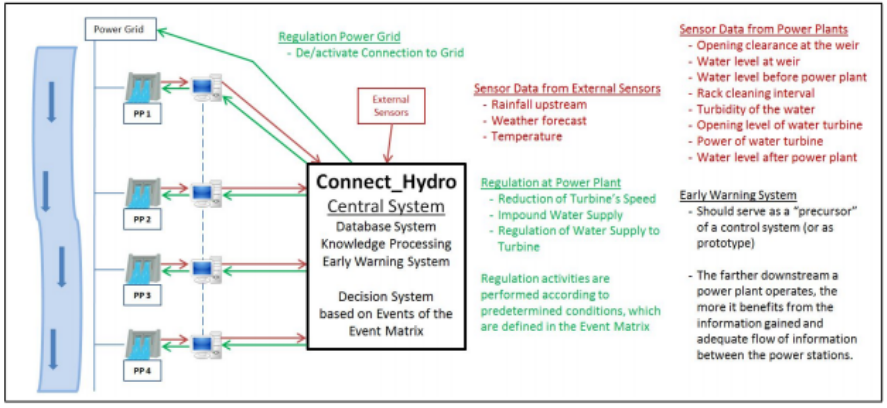
\includegraphics[scale=0.5]{Images/ConnectHydro.png}
\caption[Overview technical concept ”Connect Hydro”]{Overview technical concept ”Connect Hydro” \cite{SEIT2017}}
\end{figure}
The workflow of the prototype starts by processing the input- and historical data from the database, mapping it to the
events in the event matrix, correlating with previous events and knowledge from the knowledge processing system. In the next chapter we will discuss how the proposed system along with the already discussed Decision support techniques can optimize the power plants production efficiently and provide the owners with informed decisions as well as implement an early warnings to manage certain events.